\section{Theorie}
\label{sec:Theorie}

% In knapper Form sind die physikalischen Grundlagen des Versuches, des Messverfahrens, sowie sämtliche für die Auswertung erforderlichen Gleichungen darzustellen. (Keine Herleitung)

% (eventuell die Aufgaben)

% Der Versuchsaufbau: Beschreibung des Versuchs und der Funktionsweise (mit Skizze/Bild/Foto)

Eine sogenannte Wärmepumpe ist eine Apperatur, welche dazu genutzt wird Wärmeenergie von einem kalten in ein wärmeres Reservoir zu leiten. 
Hierzu wird zusätzliche Arbeit aufgewendet, da ansonsten Wärmeenergie immer vom warmen ins kalte Reservoir fließt.

Unter idealisierten Bedingungen wird die Güteziffer mit
\begin{equation}
    \nu = \frac{Q_1}{A} = \frac{T_1}{T_1-T_2}
    \label{eq:gueteziffer}
\end{equation}
definiert, wobei $A$ der aufgewendeten Arbeit entspricht und $Q_1$ der ans warme Reservoir abgegebenen Wärmeenergie entspricht. $T_1$ ist dabei die Temperatur im warmen und $T_2$ die im kalten Reservoir. \cite{V206}
Hier wurde vorausgesetzt dass der Wärmeübertrag reversibel geschieht, was in der Realität aber nicht möglich ist. Tatsächlich ist nur eine kleinere Güteziffer möglich.

\begin{figure}
    \centering
    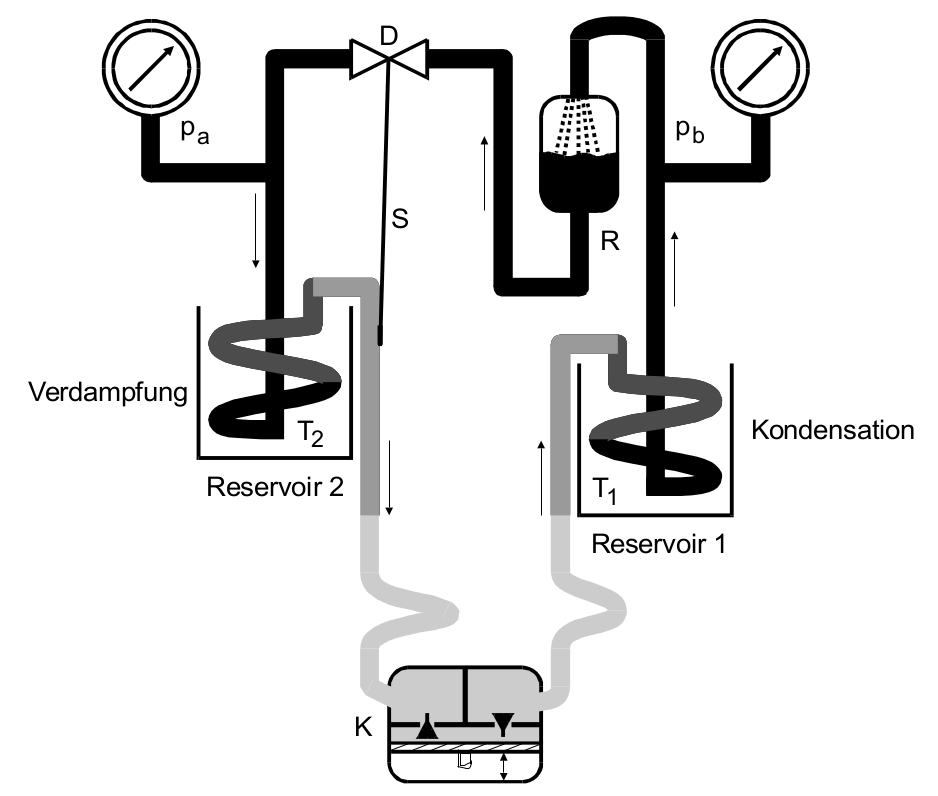
\includegraphics[width=\textwidth/2]{images/skizze_1.png}
    \caption{Schematischer Aufbau einer Wärmepumpe\cite{V206}}
    \label{fig:skizze_1}
\end{figure}

Die Wärmepumpe, wie in \autoref{fig:skizze_1} zu sehen, ist so konzipiert, dass ein Medium die Wärmeenergie beim Verdampfen im kalten Reservoir 2 als Phasenumwandlungsenergie speichert und im warmen Reservoir 1 beim Kondensieren wieder abgibt.
Da hier eine möglichst hohe Kondensationswärme des Transportmediums erforderlich ist, wird in diesem Versuch Wasser als Medium verwendet.
Das Drosselventil $D$ und der Kompressor $K$ (nahezu adiabatisch) werden dazu verwendet einen Druckunterschied $p_\text{a} < p_\text{b}$ zu erzeugen, wobei so die Verdampfung und Verflüssigung erzeugt werden.
Außerdem erkältet das Medium wenn es durch $D$ strömt und erwärmt sich wenn es durch $K$ strömt.
Zusätzlich muss noch ein Reiniger $R$ dazugeschaltet werden, welcher das flüssige Medium von Gasresten trennt. 
Außerdem wird das Drosselventil über eine Steuervorrichtung $S$ so gedrosselt, dass die Durchströmung zu der des Kompressors passt, damit in diese nur Gas strömt.

Mithilfe dieses Aufbaus kann die Güteziffer durch
\begin{equation}
    v = (m_1 c_w + m_k c_k) \frac{\Delta T_1}{\Delta t \; N}
    \label{eq:gueteziffer_2}
\end{equation}
bestimmt werden. 
Hierzu wird die Masse des Wassers in Reservoir 1 $m_1$ benötigt, die spezifische Wärmekapazität von Wasser $c_\text{w}$ und die Wärmekapazität der Rohre und der Reservoirs $m_\text{k} c_\text{k}$.
Außerdem werden die gemessenen Größen der Temperaturdifferenz $\Delta T_1$ in einem Zeitraum $\Delta t$ und die gemittelte Leistungsaufnahme des Kompressors $N$ benötigt.\cite{V206}

Über
\begin{equation}
    \frac{\Delta m}{\Delta t} = (m_2 c_\text{w} + m_\text{k} c_\text{k}) \frac{\Delta T_2}{\Delta t \; L}
    \label{eq:massen}
\end{equation}
kann der Massendurchsatz berechnet werden, wobei $L$ die Verdampfungswärme ist.

Die mechanische Leistung des Kompressors kann über
\begin{equation}
    N_\text{mech} = \frac{1}{\kappa - 1} \left( p_b \sqrt[\kappa]{\frac{p_\text{a}}{p_\text{b}}} - p_\text{a} \right) \frac{1}{\rho} \frac{\Delta m}{\Delta t}
    \label{eq:arbeit}
\end{equation}
mit dem Vehältnis $\kappa$ der Molwärmen $C_p$ und $C_V$ und der Dichte $\rho$ von Wasser im Gasförmigen Zustand bei Druck $p_a$ berechnet werden.\cite{V206}